\section{Color and Image}
\subsection{Rasterization}
For each pixel, if the center of the pixel is inside the triangle, consider it part of the triangle (and color it with the triangleʼs color.)
\subsection{Phong Reflection Model}
\[
	\begin{aligned}
		C&=
		\text{ambient}+\text{diffuse}+\text{specular}
		\\&=
		k_a+k_d\max(0,\hat{N}\cdot\hat{L})+k_s\qty(\max(0,\hat{V}\cdot\hat{R}))^\alpha
	\end{aligned}
\]
where $\hat{N}, \hat{L}, \hat{V}$ and $\hat{R}$ are defined as follows.
\begin{figure}[htpb]
	\centering
	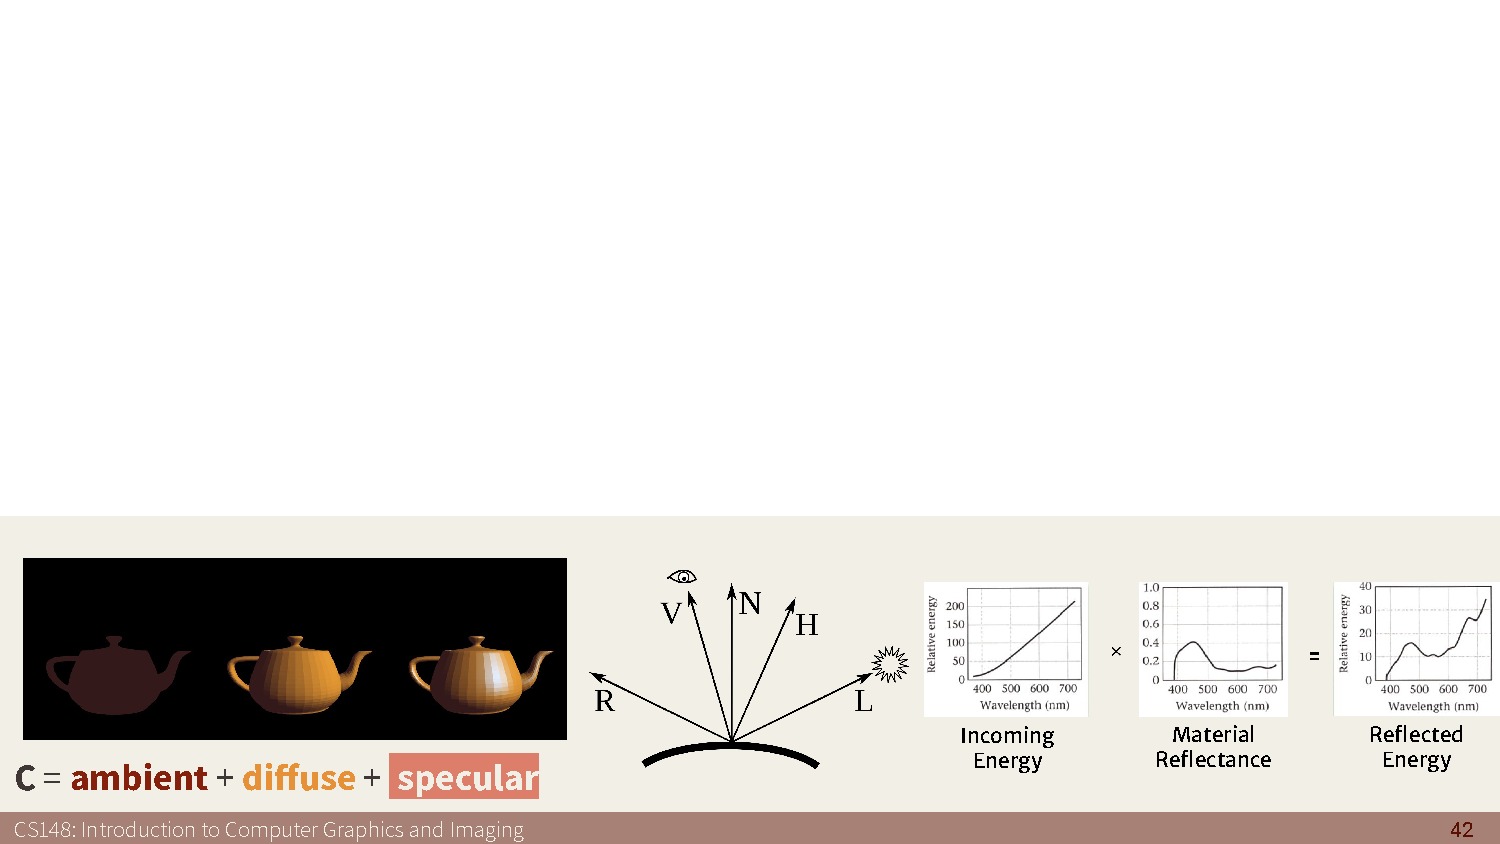
\includegraphics[width=\linewidth]{img/prm.pdf}
	\label{fig:prm}
\end{figure}
\begin{itemize}
	\vspace{-2.5em}\item \textbf{Ambient}: ``Base color''. Light bounces arounf the environment.
	\vspace{-0.5em}\item \textbf{Diffuse}: ``Rough marterial''. Given the same light source, objects look brighter when hit ``perpendicularly''.
	\vspace{-0.5em}\item \textbf{Specular}: ``Shiny material''. Bright highlights when light reflects into our eyes.
\end{itemize}
